\section{\glossaryItem{Super-Admin}}

Di seguito vengono elencati i casi d'uso per il \glossaryItem{Super-Admin}.

\newpage

\subsection{Casi d'Uso}

\subsection{UC-S0}

    \begin{figure}[h]
      \begin{center}
        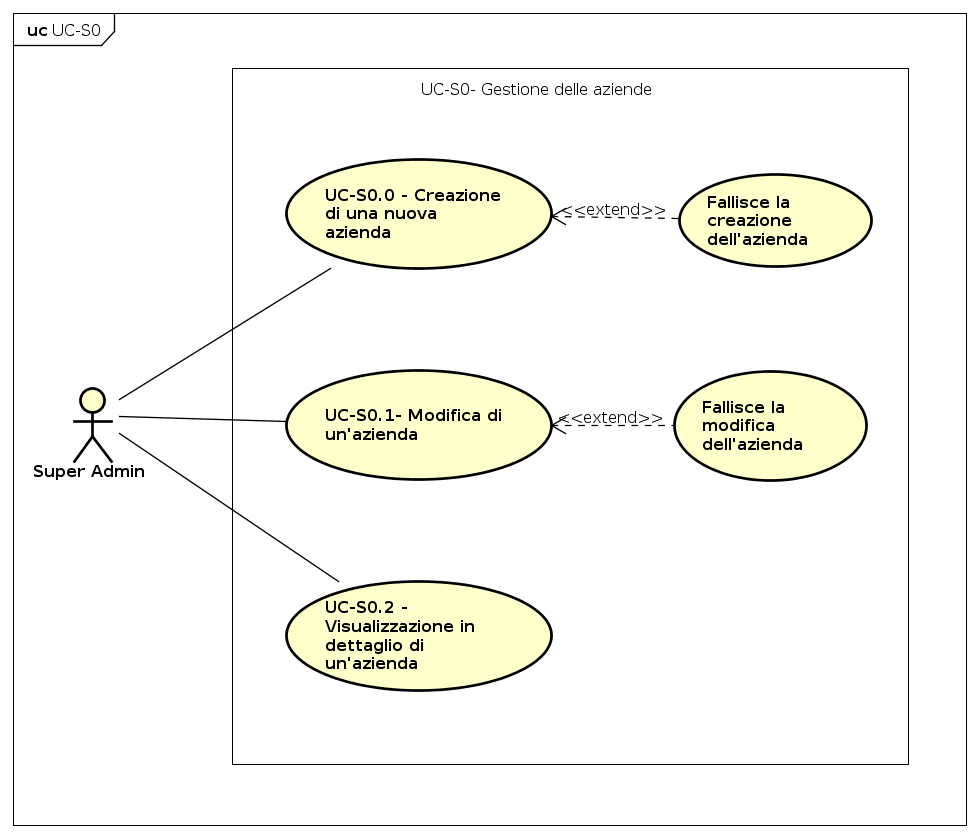
\includegraphics[width=12cm]{res/img/UCSuperadmin/UCS0.png}
      \caption{UC-S 0 - Gestione \glossaryItem{Company}}
      \end{center} 
    \end{figure}    
    
    %Tabella 
    \begin{center}
      \bgroup
      \def\arraystretch{1.8}     
      \begin{longtable}{  p{3.5cm} | p{8cm} } 
        
        \hline
        \multicolumn{2}{ | c | }{ \cellcolor[gray]{0.9} \textbf{UC-S0 - Gestione \glossaryItem{Company}}} \\ 
        \hline
        
        \textbf{Attori Primari} & \glossaryItem{Super-Admin}.\\  
        \textbf{Precondizioni}  & L'applicazione mostra al Super-Admin la pagina di gestione delle \glossaryItem{Company}.  \\ 
        
        \textbf{Postcondizioni} & L'applicazione ha dato la possibilità al Super-Admin di interagire con la pagina di gestione delle \glossaryItem{Company}. \\ 
        \textbf{Scenario principale} & 1. Il Super-Admin pu\`o creare una nuova \glossaryItem{Company}. (UC-S1) 
        
        2. Il Super-Admin pu\`o modificare i dati di una \glossaryItem{Company}. (UC-S2)  \\ 
        
        3. Il Super-Admin può visualizzare il dettaglio di una \glossaryItem{Company}. (UC-S3)
        
        \textbf{Estensioni} & 1. Fallisce l'inserimento di una nuova \glossaryItem{Company}.
        
        2. Fallisce la modifica dei dati di una \glossaryItem{Company}. \\
      \end{longtable}
      \egroup
    \end{center}

\subsection{UC-S1}
    \begin{figure}[H]
      \begin{center}
        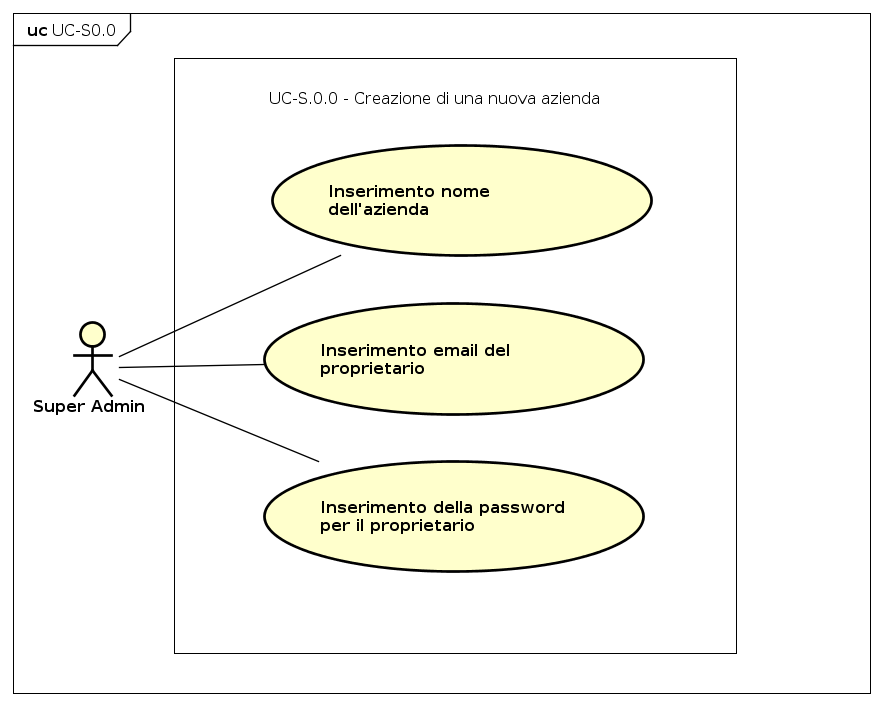
\includegraphics[width=12cm]{res/img/UCSuperadmin/UCS0.0.png}
      \caption{UC-S 0.0 - Creazione di una nuova \glossaryItem{Company}}
      \end{center} 
    \end{figure}    
    
    %Tabella 
    \begin{center}
      \bgroup
      \def\arraystretch{1.8}     
      \begin{longtable}{  p{3.5cm} | p{8cm} } 
        
        \hline
        \multicolumn{2}{ | c | }{ \cellcolor[gray]{0.9} \textbf{UC-S1 - Creazione di una nuova \glossaryItem{Company}}} \\ 
        \hline
        
        \textbf{Attori Primari} & \glossaryItem{Super-Admin}.\\  
        \textbf{Precondizioni}  & Il sistema fornisce al \glossaryItem{Super-Admin} un form di registrazione.  \\ 
        
        \textbf{Postcondizioni} & Il sistema ha aggiunto una nuova \glossaryItem{Company} e il suo \glossaryItem{Owner}. \\ 
        \textbf{Scenario principale} & 1. L'\glossaryItem{Attore} inserisce il nome della \glossaryItem{Company}.
        
        2. L'\glossaryItem{Attore} inserisce la propria email.
        
        3. L'\glossaryItem{Attore} inserisce una password \\ 
        \textbf{Estensioni} & 1. la \glossaryItem{Company} esiste gi\`a. 
        
        2. L'email inserita \`e gi\`a stata usata. \\
      \end{longtable}
      \egroup
    \end{center}

\subsection{UC-S2}
    \begin{figure}[H]
      \begin{center}
        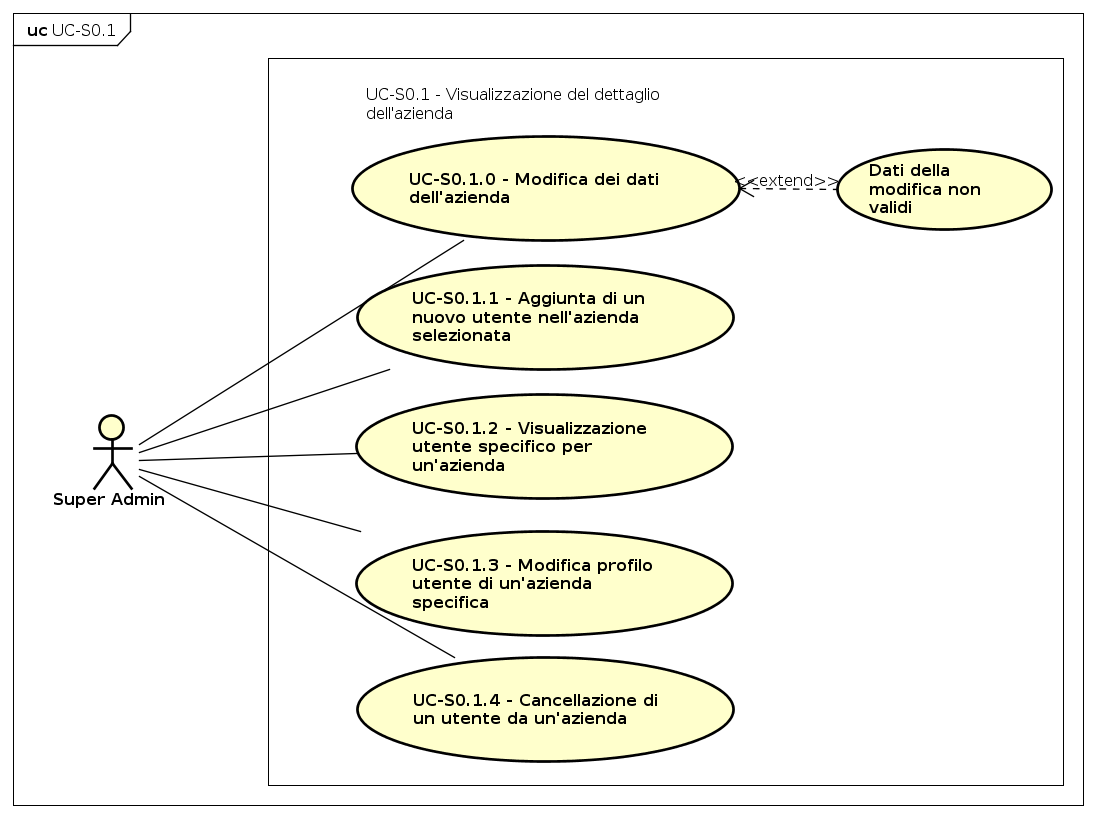
\includegraphics[width=12cm]{res/img/UCSuperadmin/UCS0.1.png}
      \caption{UC-S2 - Visualizzazione dettaglio di una \glossaryItem{Company}}
      \end{center} 
    \end{figure}    
    
    %Tabella 
    \begin{center}
      \bgroup
      \def\arraystretch{1.8}     
      \begin{longtable}{  p{3.5cm} | p{8cm} } 
        
        \hline
        \multicolumn{2}{ | c | }{ \cellcolor[gray]{0.9} \textbf{UC-S2 - Visualizzazione dettaglio di \glossaryItem{Company}}} \\ 
        \hline
        
        \textbf{Attori Primari} & \glossaryItem{Super-Admin}\\  
        \textbf{Precondizioni}  & L'applicazione mette disposizione la pagina di visualizzazione dei dettagli di una \glossaryItem{Company}.  \\ 
        
        \textbf{Postcondizioni} & L'applicazione ha reindirizzato il \glossaryItem{Super-Admin} alla pagina di visualizzazione della \glossaryItem{Company} selezionata. \\
        
        \textbf{Scenario principale} & 1. Il \glossaryItem{Super-Admin} può modificare i dati della \glossaryItem{Company}(UC-S 0.1.0);  
        
        2. Il \glossaryItem{Super-Admin} può aggiungere un nuovo utente della \glossaryItem{Company};
        
        3. Il \glossaryItem{Super-Admin} può visualizzare uno specifico utente della \glossaryItem{Company}; 
        
        4. Il \glossaryItem{Super-Admin} pu\`o modificare i dati di uno specifico utente. \\ 
        
        \textbf{Estensioni} & 1. Fallimento della modifica dei dati della \glossaryItem{Company};
        
        2. Fallimento dell'aggiunta di un nuovo utente;
        
        3. Fallimento modifica utente. \\
      \end{longtable}
      \egroup
    \end{center}


\subsection{UC-S3}
    \begin{figure}[H]
      \begin{center}
        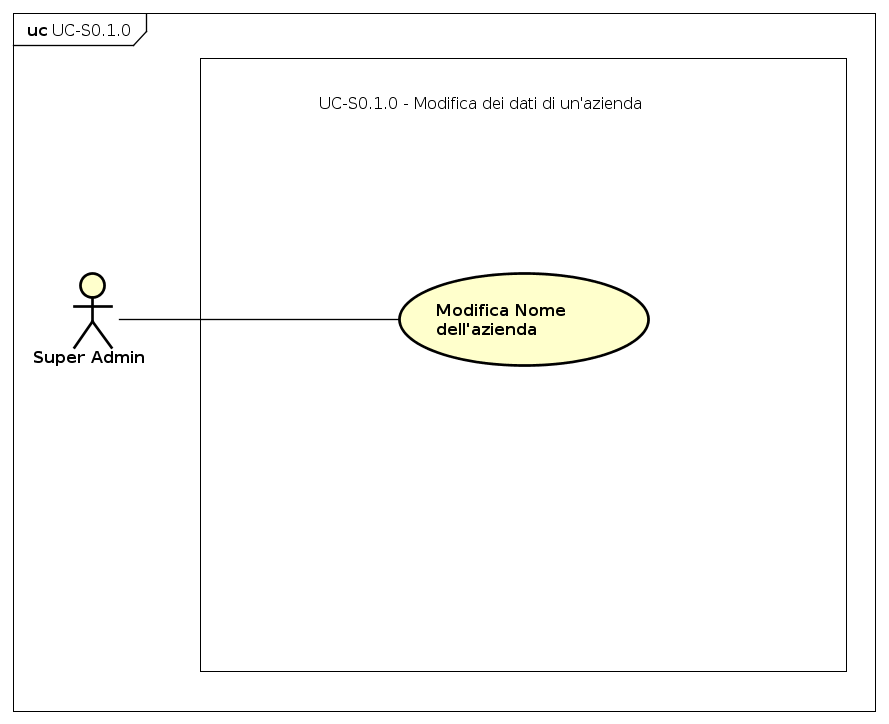
\includegraphics[width=12cm]{res/img/UCSuperadmin/UCS0.1.0.png}
      \caption{UC-S 0.1.0 - Modifica dei dati di una \glossaryItem{Company}}
      \end{center} 
    \end{figure}    
    
    %Tabella 
    \begin{center}
      \bgroup
      \def\arraystretch{1.8}     
      \begin{longtable}{  p{3.5cm} | p{8cm} } 
        
        \hline
        \multicolumn{2}{ | c | }{ \cellcolor[gray]{0.9} \textbf{UC-S 0.1.0 - Modifica dei dati di una \glossaryItem{Company}}}. \\ 
        \hline
        
        \textbf{Attori Primari} & \glossaryItem{Super-Admin}.\\  
        \textbf{Precondizioni}  & l'applicazione mostra il form per la modifica dei dati della \glossaryItem{Company} selezionata.  \\ 
        
        \textbf{Postcondizioni} & il sistema ha modificato il profilo della \glossaryItem{Company} sulla base dei dati inseriti dal \glossaryItem{Super-Admin}.  \\ 
        \textbf{Estensioni} & 1. fallimento della modifica.
      \end{longtable}
      \egroup
    \end{center}

\subsection{UC-S0.1.1}
    \begin{figure}[H]
      \begin{center}
        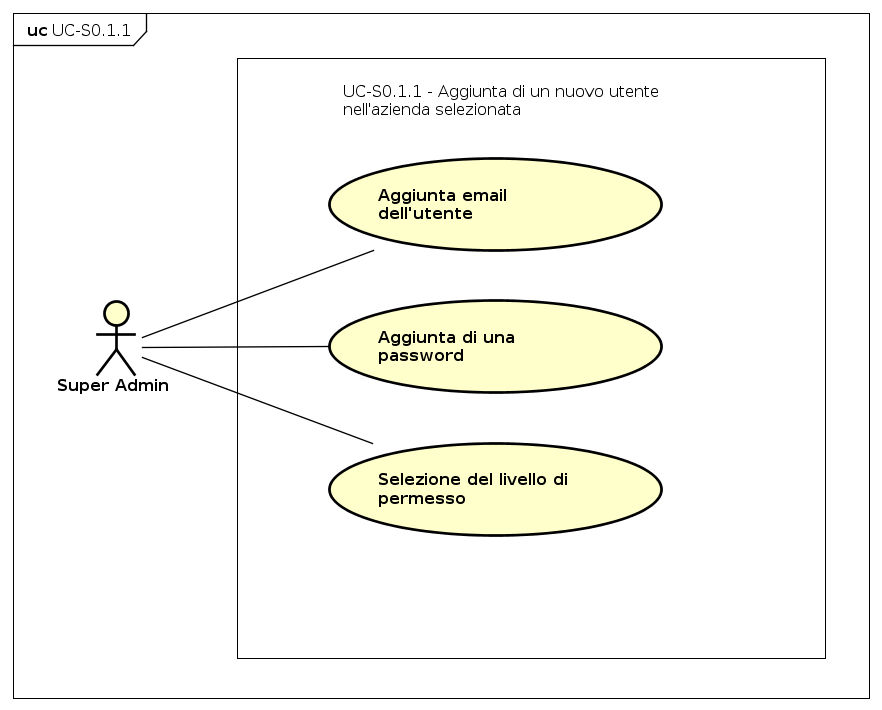
\includegraphics[width=12cm]{res/img/UCSuperadmin/UCS0.1.1.png}
      \caption{UC-S 0.1.1 - Aggiunta di un nuovo utente nella \glossaryItem{Company} selezionata}
      \end{center} 
    \end{figure}    
    
    %Tabella 
    \begin{center}
      \bgroup
      \def\arraystretch{1.8}     
      \begin{longtable}{  p{3.5cm} | p{8cm} } 
        
        \hline
        \multicolumn{2}{ | c | }{ \cellcolor[gray]{0.9} \textbf{UC-S 0.1.1 - Aggiunta di un nuovo utente nella \glossaryItem{Company} selezionata}} \\ 
        \hline
        
        \textbf{Attori Primari} & \glossaryItem{Super-Admin}.\\  
        \textbf{Precondizioni}  & l'applicazione mostra il form per l'aggiunta di un nuovo utente.  \\ 
        
        \textbf{Postcondizioni} & il sistema ha aggiunto un nuovo utente associandolo alla \glossaryItem{Company} precedentemente selezionata.  \\ 
      \end{longtable}
      \egroup
    \end{center}

\subsection{UC-S0.1.2}
    \begin{figure}[H]
      \begin{center}
        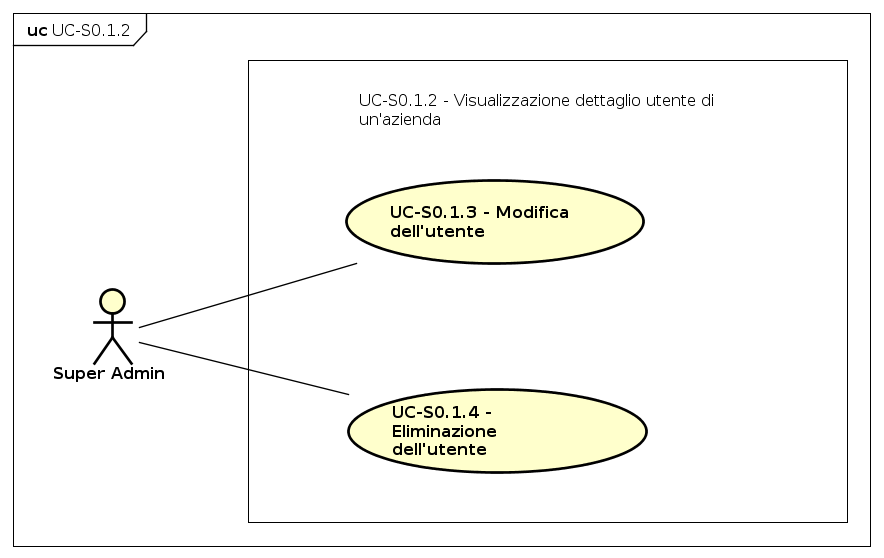
\includegraphics[width=12cm]{res/img/UCSuperadmin/UCS0.1.2.png}
      \caption{UC-S 0.1.2 - Visualizzazione in dettaglio di un utente della \glossaryItem{Company}}
      \end{center} 
    \end{figure}    
    
    %Tabella 
    \begin{center}
      \bgroup
      \def\arraystretch{1.8}     
      \begin{longtable}{  p{3.5cm} | p{8cm} } 
        
        \hline
        \multicolumn{2}{ | c | }{ \cellcolor[gray]{0.9} \textbf{UC-S 0.1.2 - Visualizzazione in dettaglio di un utente della \glossaryItem{Company}}} \\ 
        \hline
        
        \textbf{Attori Primari} & \glossaryItem{Super-Admin}\\  
        \textbf{Scopo e descrizione} & il \glossaryItem{Super-Admin} entra nella pagina di visualizzazione di un utente, nella quale pu\`o ispezionarne il profilo, inoltre pu\`o essere reindirizzato alle pagine di modifica ed eliminazione del utente in questione. \\
        \textbf{Precondizioni}  & il sistema presenta la pagina di visualizzazione in dettaglio di un utente;  \\ 
        
        \textbf{Postcondizioni} & il sistema ha ricevuto l'input dall'\glossaryItem{Attore}.  \\ 
         \textbf{Scenario principale} & 1. il \glossaryItem{Super-Admin} pu\`o modificare il profilo dell'utente; 
         
         2. il \glossaryItem{Super-Admin} pu\`o eliminare l'utente.  \\
        
     
     \end{longtable}
      \egroup
    \end{center}

\subsection{UC-S0.1.3}
    \begin{figure}[H]
      \begin{center}
        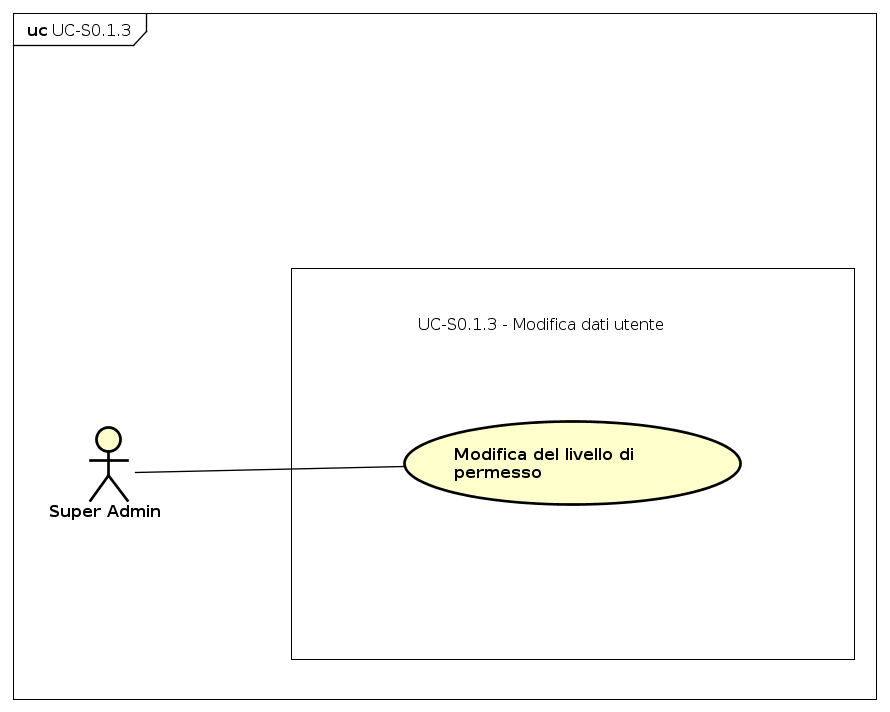
\includegraphics[width=12cm]{res/img/UCSuperadmin/UCS0.1.3.png}
      \caption{UC-S 0.1.3 - Modifica del profilo di un utente}
      \end{center} 
    \end{figure}    
    
    %Tabella 
    \begin{center}
      \bgroup
      \def\arraystretch{1.8}     
      \begin{longtable}{  p{3.5cm} | p{8cm} } 
        
        \hline
        \multicolumn{2}{ | c | }{ \cellcolor[gray]{0.9} \textbf{UC-S 0.1.3 - Modifica del profilo di un utente }} \\ 
        \hline
        
        \textbf{Attori Primari} & \glossaryItem{Super-Admin}\\  
        \textbf{Scopo e descrizione} & l'\glossaryItem{Attore} entra nella pagina di modifica dell'utente, nella quale ha la possibilit\`a
        di modificarne ruolo e password. \\
      
        \textbf{Precondizioni}  & l'applicazione predispone un form di modifica del profilo. \\ 
        
        \textbf{Postcondizioni} & il sistema ha modificato il profilo dell'utente sulla base di quanto inserito dall'\glossaryItem{Attore}. \\ 
         \textbf{Scenario principale} & 1. l'utente ha la possibilit\`a di modificare la tipologia dell'utente. \\
        
        
         \textbf{Estensioni} & 1. uscita dalla pagina senza salvataggio delle modifiche.  \\
     
     \end{longtable}
      \egroup
    \end{center}



\subsection{UC-S0.1.4}
    \begin{figure}[H]
      \begin{center}
        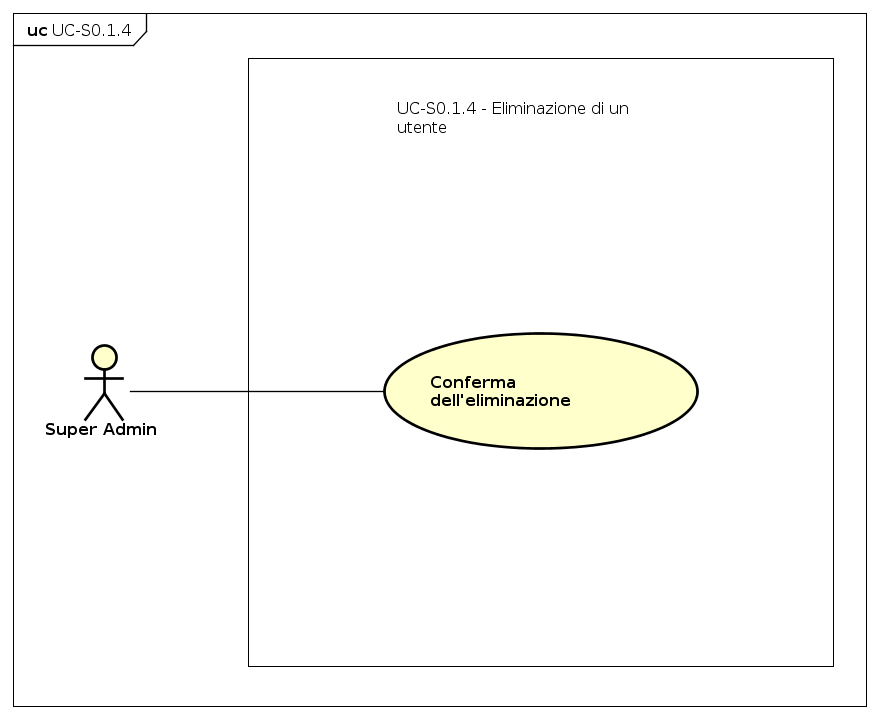
\includegraphics[width=12cm]{res/img/UCSuperadmin/UCS0.1.4.png}
      \caption{UC-S 0.1.4 - Eliminazione di un utente}
      \end{center} 
    \end{figure}    
    
    %Tabella 
    \begin{center}
      \bgroup
      \def\arraystretch{1.8}     
      \begin{longtable}{  p{3.5cm} | p{8cm} } 
        
        \hline
        \multicolumn{2}{ | c | }{ \cellcolor[gray]{0.9} \textbf{UC-S 0.1.4 - Eliminazione di un utente }} \\ 
        \hline
        
        \textbf{Attori Primari} & \glossaryItem{Super-Admin}\\  
        \textbf{Scopo e descrizione} & l'\glossaryItem{Attore} entra nella pagina di eliminazione dell'utente, nella quale ha la possibilit\`a
        di eliminarlo. \\
      
        \textbf{Precondizioni}  & l'applicazione richiede la conferma dell'eliminazione dell'utente. \\ 
        
        \textbf{Postcondizioni} & il sistema ha seguito le indicazioni dell'\glossaryItem{Attore}. \\ 
         \textbf{Scenario principale} & 1. l'\glossaryItem{Attore} ha la possibilit\`a di confermare l'eliminazione; 
         
         2. l'\glossaryItem{Attore} ha la possibilit\`a ritirare la richiesta di eliminazione. \\
        
         \textbf{Estensioni} & 1. uscita dalla pagina senza salvataggio delle modifiche.  \\
     
     \end{longtable}
      \egroup
    \end{center}


\subsection{UC-S1}
    \begin{figure}[H]
      \begin{center}
        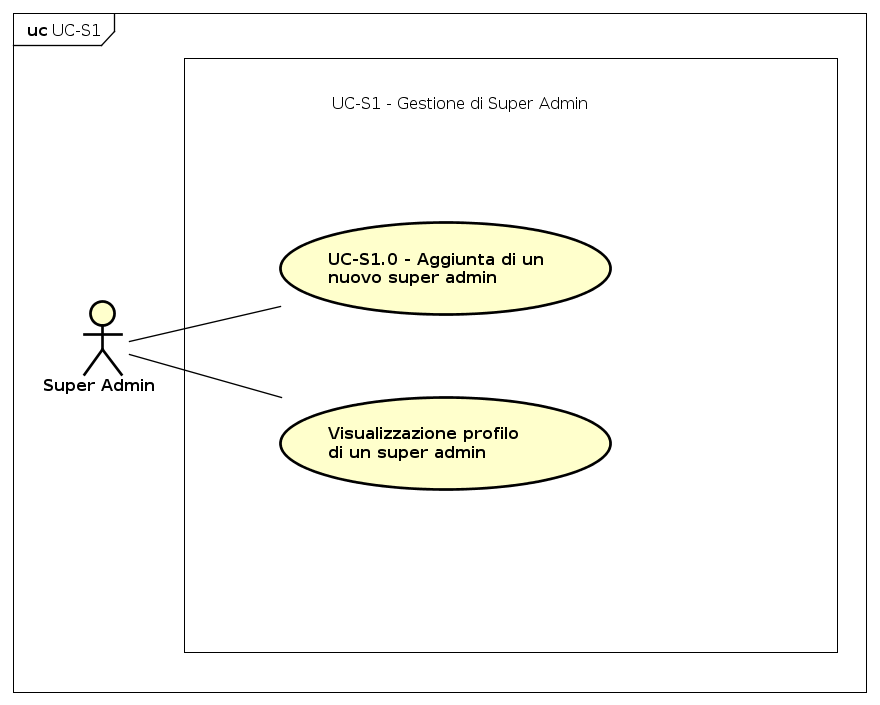
\includegraphics[width=12cm]{res/img/UCSuperadmin/UCS1.png}
      \caption{UC-S 1 - Gestione di altri \glossaryItem{Super-Admin}}
      \end{center} 
    \end{figure}    
    
    %Tabella 
    \begin{center}
      \bgroup
      \def\arraystretch{1.8}     
      \begin{longtable}{  p{3.5cm} | p{8cm} } 
        
        \hline
        \multicolumn{2}{ | c | }{ \cellcolor[gray]{0.9} \textbf{UC-S 1 - Gestione di altri \glossaryItem{Super-Admin} }} \\ 
        \hline
        
        \textbf{Attori Primari} & \glossaryItem{Super-Admin}.\\  
        \textbf{Scopo e descrizione} & L'utente è entrato nella pagina di gestione dei \glossaryItem{Super-Admin}. In questa pagina può aggiungere un nuovo \glossaryItem{Super-Admin},
vedere in un elenco quelli già presenti e poterne vedere le informazioni in dettaglio cliccando nella voce dell'elenco. \\
        \textbf{Precondizioni}  & il \glossaryItem{Super-Admin} entra nella pagina di gestione dei \glossaryItem{Super-Admin}.\\ 
        
        \textbf{Postcondizioni} & il sistema ha preso in carico le indicazioni dell'\glossaryItem{Attore}. \\ 
         \textbf{Scenario principale} & 1. l'\glossaryItem{Attore} ha la possibilit\`a di aggiungere un nuovo \glossaryItem{Super-Admin}  
         
         2. l'\glossaryItem{Attore} ha la possibilit\`a di visualizzare in dettaglio il profilo di un \glossaryItem{Super-Admin} esistente. \\
        
         \textbf{Estensioni} & 1. fallimento dell'inserimento di un \glossaryItem{Super-Admin}.  \\
     
     \end{longtable}
      \egroup
    \end{center}


\subsection{UC-S1.0}
    \begin{figure}[H]
      \begin{center}
        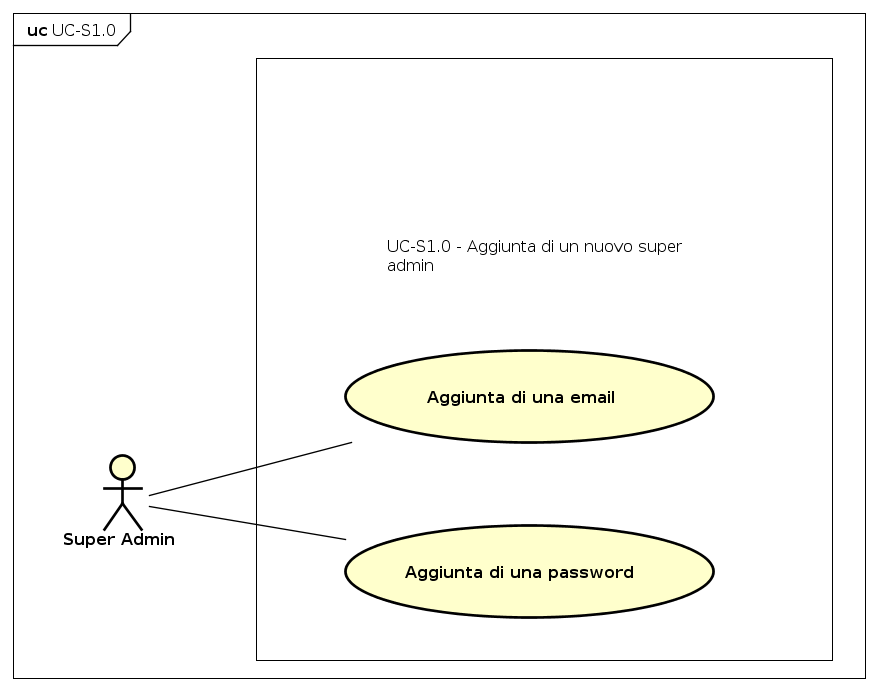
\includegraphics[width=12cm]{res/img/UCSuperadmin/UCS1.0.png}
      \caption{UC-S 1.0 - Creazione di un \glossaryItem{Super-Admin}}
      \end{center} 
    \end{figure}    
    
    %Tabella 
    \begin{center}
      \bgroup
      \def\arraystretch{1.8}     
      \begin{longtable}{  p{3.5cm} | p{8cm} } 
        
        \hline
        \multicolumn{2}{ | c | }{ \cellcolor[gray]{0.9} \textbf{UC-S 1.0 - Creazione di un \glossaryItem{Super-Admin} }} \\ 
        \hline
        
        \textbf{Attori Primari} & \glossaryItem{Super-Admin}.\\  
        \textbf{Scopo e descrizione} & l'\glossaryItem{Attore} entra nella pagina di creazione di un altro \glossaryItem{Super-Admin}. 
        Qui deve aggiungere le informazioni (email, password) necessarie per la registrazione di un nuovo \glossaryItem{Super-Admin}. \\
      
        \textbf{Precondizioni}  &  l'\glossaryItem{Attore} entra nella pagina di creazione di un nuovo \glossaryItem{Super-Admin} \\
        \textbf{Postcondizioni} & il sistema ha creato un nuovo \glossaryItem{Super-Admin} nel database \\ 
         \textbf{Scenario principale} & 1. l'\glossaryItem{Attore} inserisce l'email dell'utente da registrare; 
         
         2. l'\glossaryItem{Attore} aggiunge una password nell'apposito campo.\\
        
         \textbf{Estensioni} & 1. l'\glossaryItem{Attore} esce dalla pagina;  
         
         2. l'email inserita \`e gi\`a presente nel database e il nuovo \glossaryItem{Super-Admin} non pu\`o essere creato.\\ 
     
     \end{longtable}
      \egroup
    \end{center}



